\section{Introduction}
Nowadays, Internet-of-Things (IoT) technologies have been used in many different fields (e.g., smart home and smart
campus) for providing convenience and efficiency to users. Similarly, this paper proposes an automatic attendance system
different from existing attendance systems. The existing attendance systems are usually operated by a manual methodor
elec-trical system by identifying a student identification (ID) card or using an attendance application. There are some
problems in these systems.
For example, there is lecture time loss because of checking attendance by a manual method.
Also, if students use an electrical attendance system, they always need to carry their student ID card or smartphone with
an attendance application. A proxy at- tendance (i.e., attendance of somebody else for the sake of a person) can be done
by an unconscionable person. This weak point of the existing attendance systems should be prevented
Maintaining the attendance is very important in all the institutes for checking the performance of employees. Every
institute has its own method in this regard. Some are taking attendance manually using the old paper or file based approach
and some have adopted methods of automatic attendance using some bio-metric techniques.
But in these methods employees have to wait for long time in making a queue at time they enter the office. Many biometric systems are available but the key au-thenti cations are same is all the techniques.
Our system uses the face recognition approach for the automatic attendance of employees in the office room environment
without employees’ intervention Face recognition consists of two steps, in first step faces are detected in the image and
then these detected faces are compared with the database for verification. A num- ber of methods have been proposed for
face detection i.e. Ada Boost algorithm, the Float Boost algorithm, the S-Ada Boost algorithm Support Vector Machines
(SVM), and the Bayes classifier
\section{COMPONENT DESCRIPTION
}
\section{Landing Page :}
This is basically the Home page of our Project. After opening the system this is the first page user will see. In this the
user can able to Register, By adding First Name, Last Name, Address, Status and mobile number. Once user submitted
his data, then we have to create our face data and train it. Then user can mark his attendance by clicking on the button
called face attendance.
And once attendance has been marked successfully, user’s care taker got notification on email.

\section{Register:}

This page provides the facility for the user to register and create a new account for only one time. This system provides
options of status so that user can register as an instructor or as a student. For registering, any user requires to fill-up the
following form box of First Name, Last Name, Address, Status and Mobile Number.
There are validations added for this form such as the Display, Soo user can Re-check he is registered successfully or not.
Also he can take look on the personal information has been submitted
         



\section{Create Face Data :}
This page basically helps to capture or create the image data set. At a time, it takes 24 images of every user by different
angels. Soo user don’t need to wait or pass through front of camera everytime .
Also We can add User Id for every user at the time of creating face data.

\section{Train Face Data :}
This Page Train the face data, that we created already. Every Time when we added new user data, This programming
page train, identify, manage all stored data. It can neglect the unwanted things from images , and crop, reduce the size of
images and soo on



\section{ALGORITHM :}
{Haar Cascade Algorithm :} Haar Cascade is a feature-based object detection algorithm to detect objects from images. A cascade function is trained
on lots of positive and negative images for detection. The algorithm does not require extensive computation and can run
in real-time
In this article, we are going to see how to detect faces using a cascade classifier in OpenCV Python. Face detection has
much significance in different fields of today’s world. It is a significant step in several applications, face recognition
(also used as biometrics), photography (for auto-focus on the face), face analysis (age, gender, emotion recognition),
video surveillance, etc
One of the popular algorithms for facial detection is “haarcascade”. It is computationally less expensive, a fast
algorithm, and gives high accuracy.

\section{Haar-feature selection:}A Haar-like feature consists of dark regions and light regions. It produces a single value by taking the difference of
the sum of the intensities of the dark regions and the sum of the intensities of light regions. It is done to extract
useful elements necessary for identifying an object. The features proposed 

\includegraphics [width=0.9\textwidth]{report.png}


\section{Creation of Integral Images:}
A given pixel in the integral image is the sum of all the pixels on the left and all the pixels above it. Since the
process of extracting Haar-like features involves calculating the difference of dark and light rectangular regions, the
introduction of Integral Images reduces the time needed to complete this task significantly

\section{AdaBoost Training:}This algorithm selects the best features from all features. It combines multiple “weak classifiers” (best features) into
one “strong classifier”. The generated “strong classifier” is basically the linear combination of all “weak classifiers”.



\section{Cascade Classifier:}
It is a method for combining increasingly more complex classifiers like AdaBoost in a cascade which allows
negative input (non-face) to be quickly discarded while spending more computation on promising or positive facelike regions. It significantly reduces the computation time and makes the process more efficient.
OpenCV comes with lots of pre-trained classifiers. Those XML files can be loaded by cascade Classifier method of
the cv2 module. Here we are going to use haarcascade_frontalface_default. xml for detecting faces.


\section{Stepwise Implementation:
}
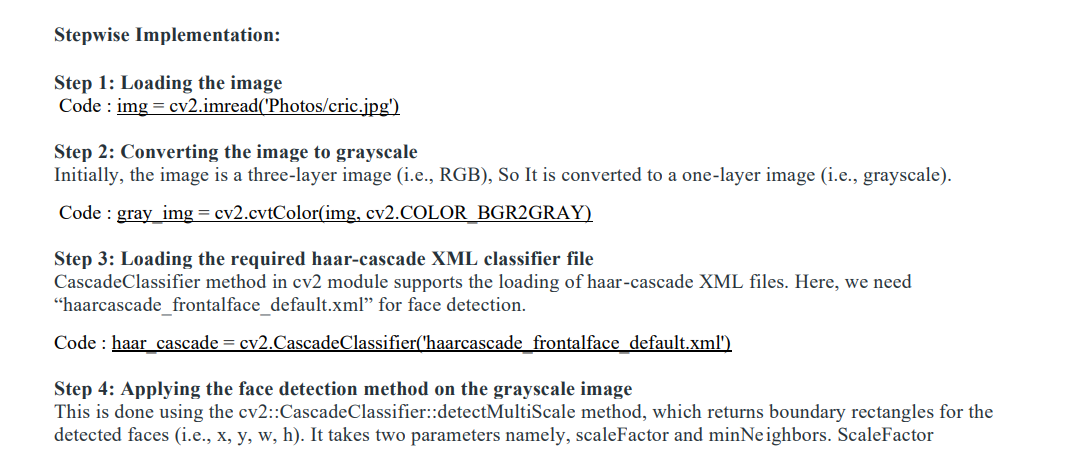
\includegraphics[width=1.3\textwidth]{step.png}
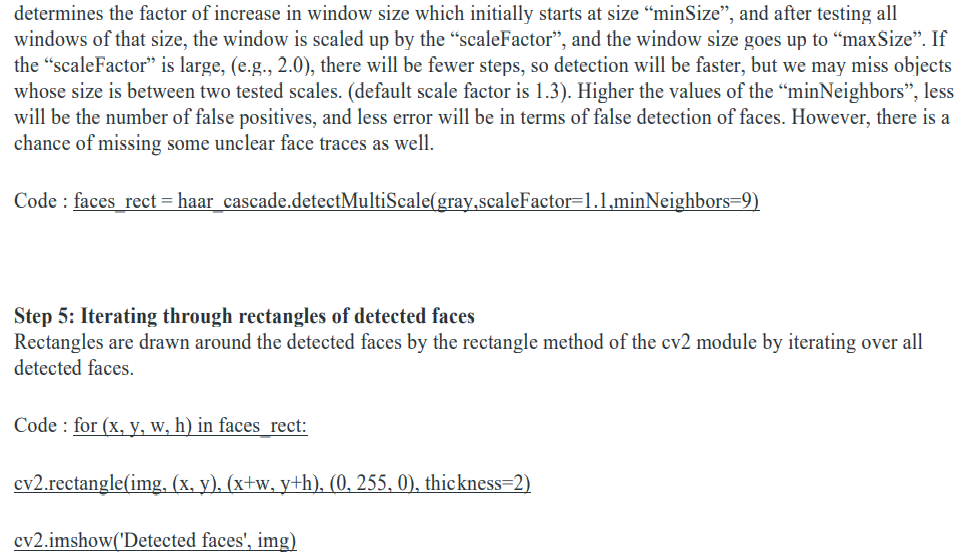
\includegraphics[width=1.3\textwidth]{step2.png}



\section {Below is the implementation :}


\includegraphics [width=0.9\textwidth]{pic.png}\\
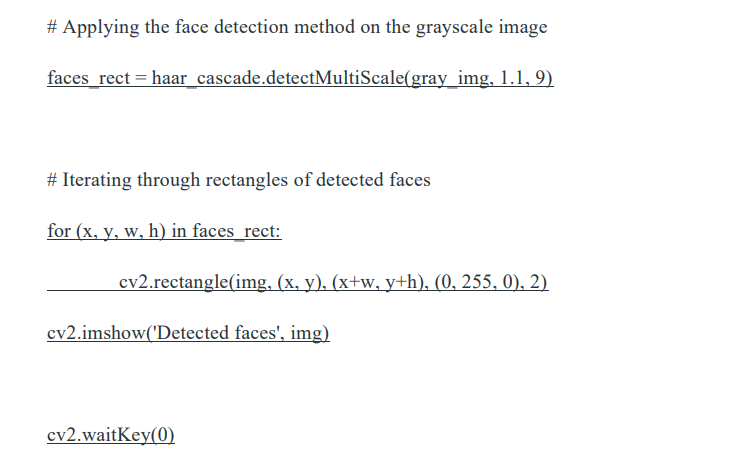
\includegraphics[width=0.9\textwidth]{pro.png}

\section {CONCLUSION}
The aim is to automate and make a system that is useful to the organization such as an institute. The efficient and accurate
method of attendance in the office environment that can replace the old manual methods. This method is secure enough,
reliable and available for use.
No need for specialized hardware for installing the system in the office. It can be constructed using a camera and
computer. Human face detection can be used in different fields, such as in law enforcement, equity arrangements,
identification recovery, and Biometrics.
Facial identity and recognition technology integrate university campus tech solutions to ensure student protection. For
chosen locations, such as university campuses, we establish facial recognition based on face detection.
Our primary point is to identify and throw unwanted persons out of the protected area. We are eager to develop a quick
and efficient framework of facial recognition that identifies and does not reach people's faces.
By calculating the illegal movement of outsiders by using our suggested methodology, we will minimize internal campus
crimes much as our point is to expand transparent mindfulness, human protection, and authorization of the law by
adopting our proposal. In the future we will add artificial intelligence over the proposed system, to differentiate
objects like humans, animals, and so on to ensure security surveillans

\section {REFERENCES}
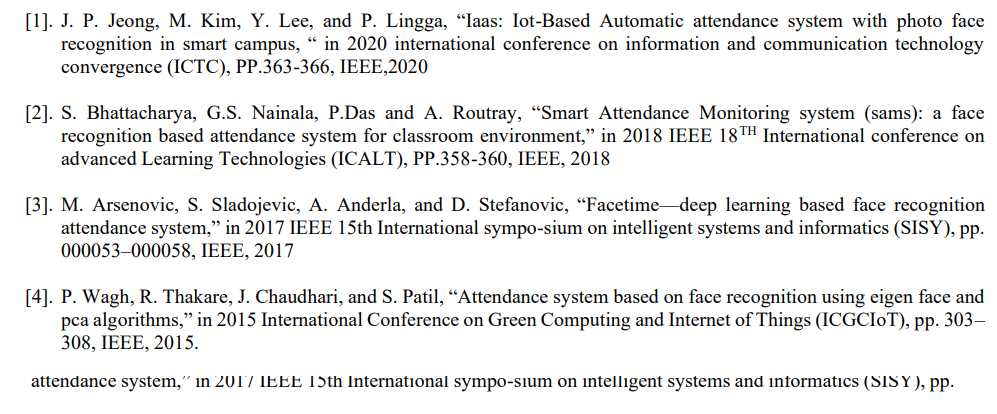
\includegraphics[width=0.9\textwidth]{ref.png}\\
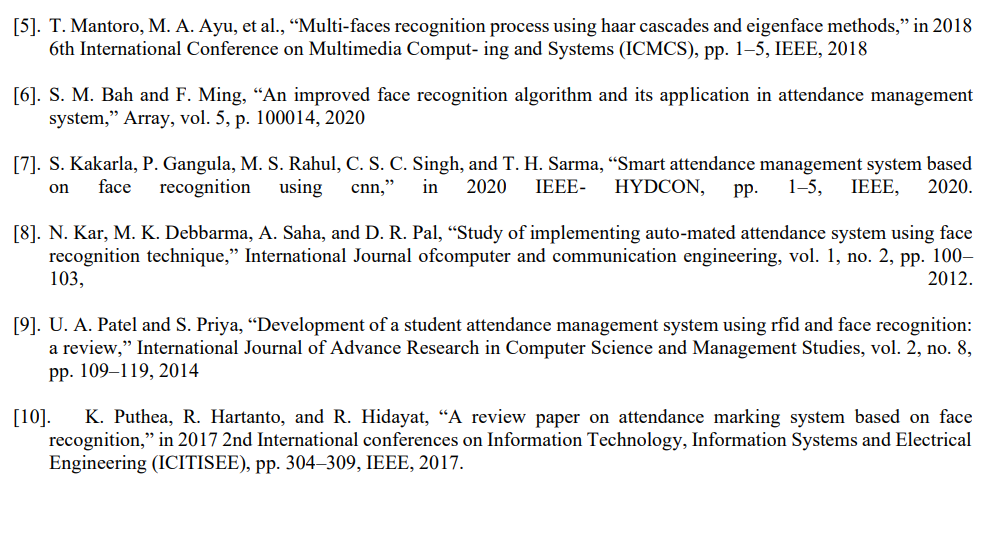
\includegraphics[width=0.9\textwidth]{ref2.png}



